
%(BEGIN_QUESTION)
% Copyright 2008, Tony R. Kuphaldt, released under the Creative Commons Attribution License (v 1.0)
% This means you may do almost anything with this work of mine, so long as you give me proper credit

Many industries produce flammable waste products that may be used as fuel in furnaces, steam boilers, and process heaters.  If this ``waste fuel'' is a gas rather than a liquid, we may collect it in a large pressure vessel (called a ``receiver'') and control the pressure within that vessel so that all the combustion processes receive fuel gas at a steady pressure.  

If we have a surplus of waste fuel coming in to the receiver vessel, the pressure will rise above setpoint.  In this event, a pressure control system opens up a control valve to vent excess fuel gas to the flare (a continuously-burning ``torch'' where waste products may be safely disposed of) to maintain receiver pressure at setpoint.  Conversely, if we aren't getting enough waste fuel coming in to the receiver vessel to meet the demands of all the combustion processes, the pressure will drop below setpoint.  In this event, the same pressure control system opens up a different control valve to introduce natural gas to the receiver vessel and bring the pressure back up to setpoint:

$$\includegraphics[width=15.5cm]{i03221x01.eps}$$

Explain how the two control valves, PV-a and PV-b, may be {\it split-ranged} so that a single pressure controller operates both valves simultaneously.  Assuming a direct-acting transmitter and reverse-acting controller (that output 4-20 mA each), determine the calibration range for each control valve.

\underbar{file i03221}
%(END_QUESTION)





%(BEGIN_ANSWER)

This application requires {\it exclusive} split-ranging:

$$\includegraphics[width=15.5cm]{i03221x02.eps}$$
 
%(END_ANSWER)





%(BEGIN_NOTES)

Increasing receiver pressure causes the reverse-acting controller output to decrease.  This causes PV-a (vent valve) to open up while PV-b (natural gas make-up valve) shuts off.  It is important that both valves be closed at 50\% output signal (12 mA) so that we don't waste natural gas by passing it straight through the receiver vessel on to the flare!

%INDEX% Final Control Elements, valve: split ranging

%(END_NOTES)


